\documentclass[12pt,a4paper]{article}

% =================================================
% LANGUAGE AND TYPOGRAPHY
% =================================================
\usepackage[T1]{fontenc}
\usepackage[utf8]{inputenc}
\usepackage[english]{babel}
\usepackage{lmodern}
\usepackage{microtype}

% =================================================
% PAGE SETUP
% =================================================
\usepackage[
    a4paper,
    top=2.7cm,
    bottom=2.5cm,
    left=2.7cm,
    right=2.7cm,
    headheight=16pt
]{geometry}

\usepackage{setspace}
\setstretch{1.15}
\setlength{\parindent}{0pt}
\setlength{\parskip}{6pt}

% =================================================
% COLORS AND HEADINGS
% =================================================
\usepackage{xcolor}
\definecolor{bleufonce}{HTML}{17365D}
\definecolor{bleuclair}{HTML}{DCE6F1}
\definecolor{gris}{HTML}{313131}

\usepackage{titlesec}

\titleformat{\section}
  {\Large\bfseries\color{bleufonce}}
  {\thesection.}{0.7em}{}
  [\vspace{3pt}\color{bleuclair}\titlerule]

\titleformat{\subsection}
  {\large\bfseries\color{bleufonce}}
  {\thesubsection}{0.7em}{}

\titlespacing*{\section}{0pt}{24pt}{12pt}
\titlespacing*{\subsection}{0pt}{16pt}{8pt}

% =================================================
% IMAGES AND LINKS
% =================================================
\usepackage{graphicx}
\usepackage{float}
\usepackage{hyperref}
\usepackage{placeins}

\hypersetup{
    colorlinks=true,
    linkcolor=bleufonce,
    urlcolor=bleufonce,
    pdftitle={C++ Mid-Project Report},
    pdfauthor={Raïan CHOUIREF and Dorian LEON FERNANDES}
}

% =================================================
% HEADERS AND FOOTERS
% =================================================
\usepackage{fancyhdr}

\pagestyle{fancy}
\fancyhf{}

\fancyhead[L]{\small\textcolor{gris}{C++ Mid-Project Report}}
\fancyhead[R]{\small\textcolor{gris}{3D Modeler}}

\fancyfoot[L]{\small\textcolor{gris}{Raïan CHOUIREF -- Dorian LEON FERNANDES}}
\fancyfoot[R]{\small\textcolor{gris}{Page \thepage}}

\renewcommand{\headrulewidth}{0.4pt}
\renewcommand{\footrulewidth}{0.4pt}

% =================================================
% TABLE OF CONTENTS
% =================================================
\usepackage{tocloft}

\renewcommand{\contentsname}{Contents}
\renewcommand{\cftsecfont}{\bfseries\color{bleufonce}}
\renewcommand{\cftsecpagefont}{\bfseries\color{bleufonce}}
\setlength{\cftbeforesecskip}{8pt}

% =================================================
% DOCUMENT
% =================================================
\begin{document}

% =================================================
% COVER PAGE
% =================================================
\begin{titlepage}
    \thispagestyle{empty}

    \centering

    \vspace*{2cm}

    {\Large\textcolor{gris}{MID-PROJECT REPORT}\par}

    \vspace{1.5cm}

    {\color{bleufonce}\rule{\textwidth}{1.5pt}\par}

    \vspace{0.7cm}

    {\Huge\bfseries C++ Report\par}

    \vspace{0.5cm}

    {\Large\textcolor{gris}{Data Structures and 3D Rendering}\par}

    \vspace{0.7cm}

    {\color{bleufonce}\rule{\textwidth}{1.5pt}\par}

    \vspace{2.5cm}

    {\large\textbf{Prepared by}\par}

    \vspace{0.5cm}

    {\Large Raïan CHOUIREF\par}
    \vspace{0.2cm}
    {\Large Dorian LEON FERNANDES\par}

    \vfill

    {\large Academic Year: 2026--2027\par}

    \vspace{0.5cm}

    {\large \today\par}

    \vspace{1cm}

\end{titlepage}

% =================================================
% TABLE OF CONTENTS
% =================================================
\pagenumbering{roman}

\tableofcontents

\newpage

% =================================================
% CONTENT
% =================================================
\pagenumbering{arabic}

\section{Introduction}

This project consists of developing a 3D editor capable of loading, displaying, and manipulating 3D models from files in .PLY and .OBJ formats. 
The main objective is to allow the user to interact with 3D models intuitively and efficiently. 
To achieve this, we need to implement a suitable data structure to represent 3D meshes, as well as a high-performance rendering system using OpenGL. 
The major steps of the project include designing the Halfedge data structure, developing the file loader, implementing the rendering system, and creating a user interface.

\section{Problem Statement}

In this project, we address the challenge of manipulating and rendering 3D models from .PLY and .OBJ files. The primary goal is to build a 3D editor that can load these files, display the corresponding models, and enable user interaction. 
The specific objectives of the project include:
\begin{itemize}
    \item Setting up an efficient data structure to represent 3D meshes, specifically using the Halfedge structure.
    \item Developing a rendering system using OpenGL to display 3D models realistically and efficiently.
    \item Creating a file loader capable of reading .PLY and .OBJ formats, extracting geometric information, and converting it into data structures usable by the program.
\end{itemize}

\newpage
\section{Project Context}

As part of the Computer Science course, we were tasked with carrying out a C++ project focused on programming and geometry. The main objective was to develop a 3D editor capable of loading, displaying, and manipulating 3D models from .PLY and .OBJ files. 
To accomplish this, we used several tools and libraries, notably OpenGL for graphical rendering, alongside tailored data structures to represent 3D meshes. 
The project constraints included managing geometric data efficiently, providing an intuitive user interface, and ensuring compatibility with various 3D file formats. We also had to ensure that our editor could handle complex models while maintaining optimal performance.

So far, we have successfully implemented basic features, including loading .PLY and .OBJ files and rendering 3D models. However, further improvements are still needed, particularly regarding performance optimization and adding extra features to enrich the user experience.

\newpage

\section{UML Architecture}

\begin{figure}[H]
    \centering
    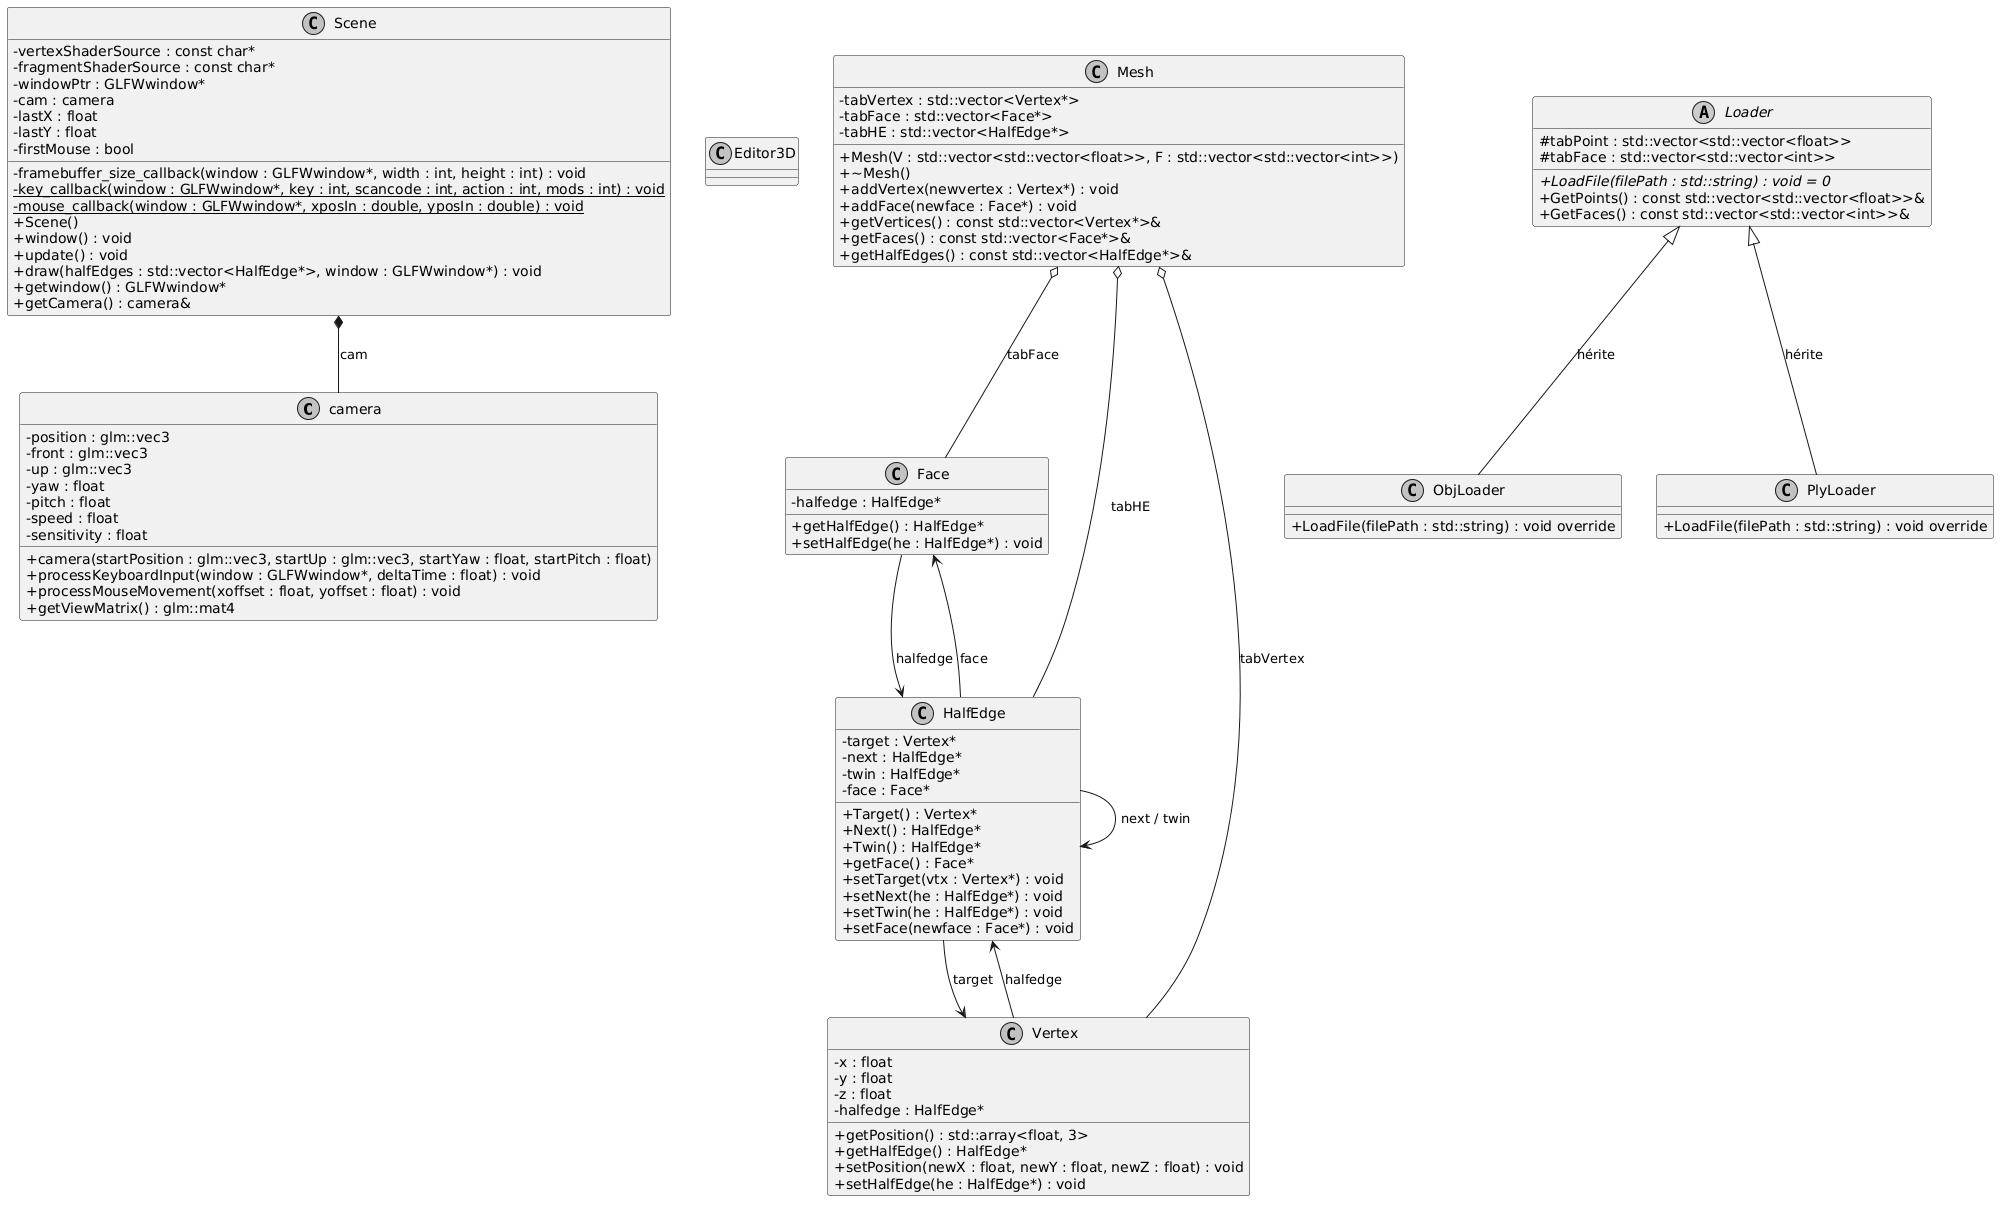
\includegraphics[width=1\textwidth]{uml.png}
    \caption{Project UML Diagram}
    \label{fig:uml}
\end{figure}

We used a UML diagram to represent the classes and their relationships within our project. The diagram illustrates the main classes, their attributes and methods, as well as their associations. This helped us better understand the project architecture and facilitated communication among team members. 

Here is an overview of the main classes and their relationships:
\begin{itemize}
    \item The \texttt{Scene} class represents the 3D scene and contains objects such as meshes and cameras. It handles rendering management and user interaction with objects.
    \item The \texttt{Mesh} class represents a 3D mesh and stores information about vertices, faces, and edges. It manages geometric data and generates data structures required for rendering.
    \item The \texttt{Halfedge} class represents a data structure for meshes, enabling efficient navigation between vertices, edges, and faces. It facilitates mesh modification and rendering operations.
\end{itemize}

\begin{figure}[H]
    \centering
    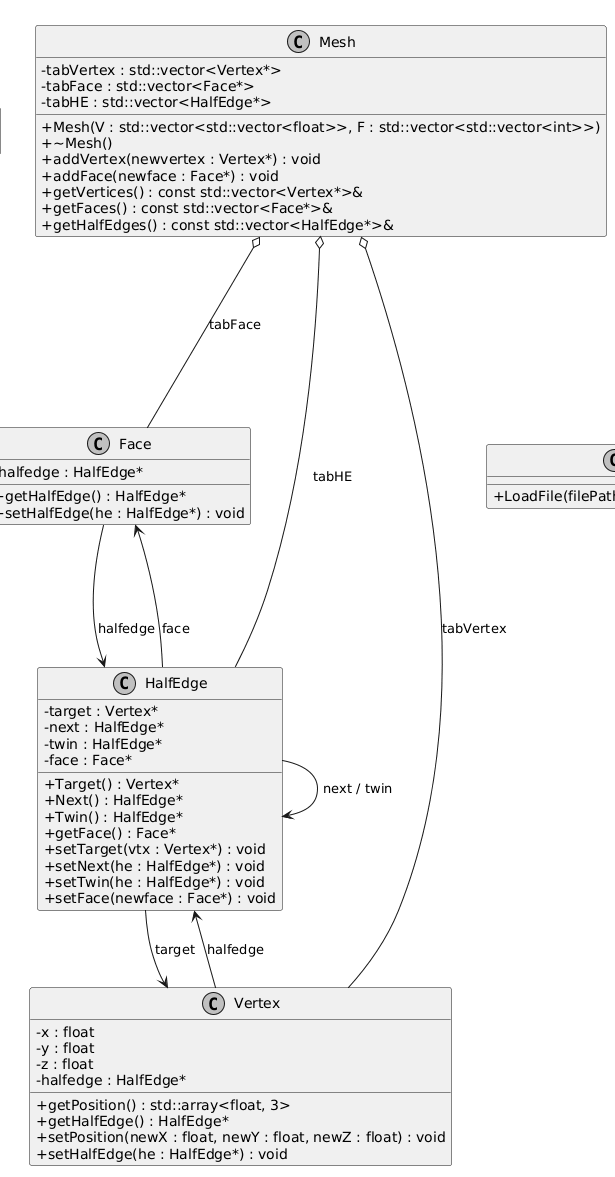
\includegraphics[width=0.55\textwidth]{mesh.png}
    \caption{UML Diagram of the Mesh Structure}
    \label{fig:uml_mesh}
\end{figure}

This section shows the UML diagram of the \texttt{Mesh} structure, representing a 3D mesh. The \texttt{Mesh} class contains attributes to store vertices, faces, and edges, along with methods to manage them. Relationships between classes are also shown, demonstrating how they interact to form the overall project architecture.

\begin{figure}[H]
    \centering
    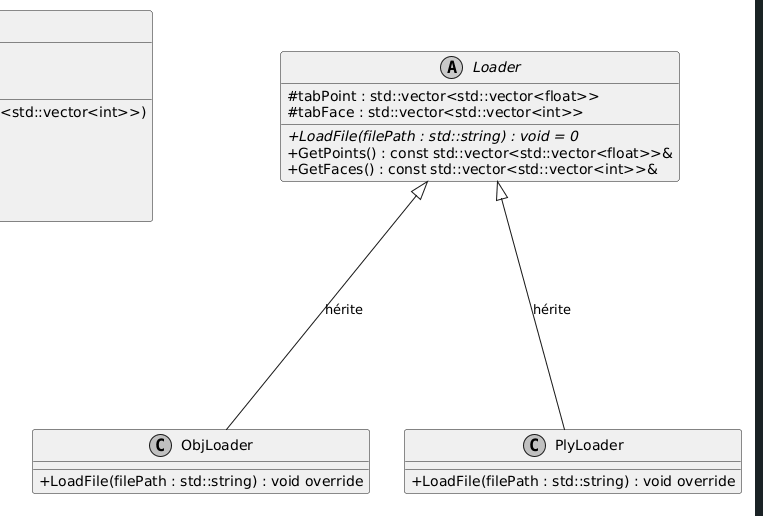
\includegraphics[width=0.55\textwidth]{loader.png}
    \caption{UML Diagram of the Loader}
    \label{fig:uml_loader}
\end{figure}

For the loader, we used a generic class design to support loading multiple file formats. 
This allowed us to create specific classes for each file format, such as \texttt{PLYLoader} and \texttt{OBJLoader}, which inherit from the generic \texttt{Loader} class. This architecture makes it straightforward to add new file formats in the future.

\newpage
\section{Loader}

The file loading system in our project relies on two specific classes, \texttt{PlyLoader} and \texttt{ObjLoader}, both inheriting from the generic \texttt{Loader} class.

The \texttt{PlyLoader} class loads \texttt{.ply} files encoded in either ASCII or Little Endian binary format. It begins by reading the header to determine the file format, vertex count, face count, data types used (\texttt{double}, \texttt{float}, \texttt{int}), and potential extra properties like color or opacity. 
Implementing this loader required handling bytes to be skipped during binary reading, such as padding or unused properties. We leveraged AI tools like ChatGPT to implement this logic and discover suitable C++ utilities like \texttt{std::istringstream}, which simplifies parsing ASCII data.

The \texttt{ObjLoader} class handles \texttt{.obj} files. It parses each line based on its prefix to distinguish vertices (identified by \texttt{v}) from faces (identified by \texttt{f}). Using \texttt{std::istringstream} allows for clean extraction of the values on each line.

Finally, both classes store extracted data into two main arrays: \texttt{tabPoint} and \texttt{tabFace}. The first contains vertex coordinates as a \texttt{std::vector<Eigen::Vector3d>}, while the second contains faces as a \texttt{std::vector<std::vector<int>>}. This organization represents vertices and connectivity in structures directly usable by the rest of the application.

\newpage
\section{Halfedge Data Structure}

Our Halfedge structure relies on three closely related classes: \texttt{Vertex}, \texttt{Face}, and \texttt{HalfEdge}.

The \texttt{Vertex} class represents mesh vertices. Each vertex stores a position as an \texttt{Eigen::Vector3d} and a pointer to an associated \texttt{HalfEdge*}.

The \texttt{Face} class represents triangular mesh faces. It contains a pointer to one of its constituent \texttt{HalfEdge} objects (\texttt{HalfEdge*}). Other halfedges belonging to the face can then be traversed via their internal links.

The \texttt{HalfEdge} class is the core of this data structure. Each halfedge contains several pointers describing its position within the mesh: a pointer to its target vertex (\texttt{Vertex*}), a pointer to the next halfedge (\texttt{next}), a pointer to its opposite twin halfedge (\texttt{twin}), and a pointer to its parent face (\texttt{Face*}).

These links allow efficient traversal of the mesh and quick access to neighboring elements. They are designed to facilitate geometric and topological modifications, though these editing features are not yet fully implemented.

The mesh structure is generated by the \texttt{Mesh} class using the vertex and face arrays provided by the loader. Elements are then organized into three arrays: \texttt{tabVertex}, \texttt{tabFace}, and \texttt{tabHE}, storing vertices, faces, and halfedges respectively.

\newpage

\section{Rendering}

For rendering, we used the \texttt{OpenGL} library, a powerful and flexible graphics API for 2D and 3D rendering. OpenGL allows us to create interactive 3D scenes and manage transformations, lighting, and textures.

Below are the vertices of a cube used to test rendering in our 3D editor:
\begin{figure}[H]
    \centering
    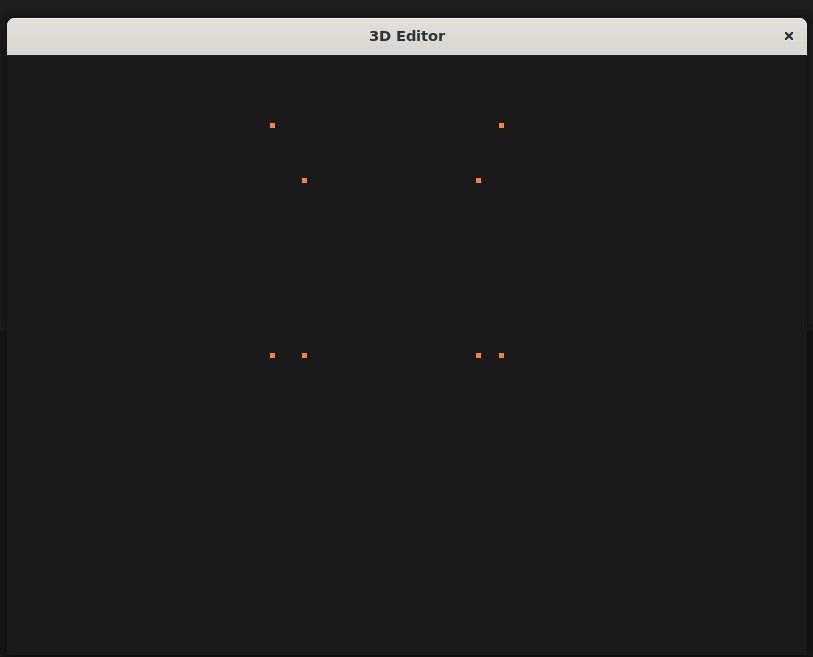
\includegraphics[width=0.5\textwidth]{point.jpeg}
    \caption{Cube vertices for rendering tests}
    \label{fig:cube}
\end{figure}

And the corresponding triangular faces:
\begin{figure}[H]
    \centering
    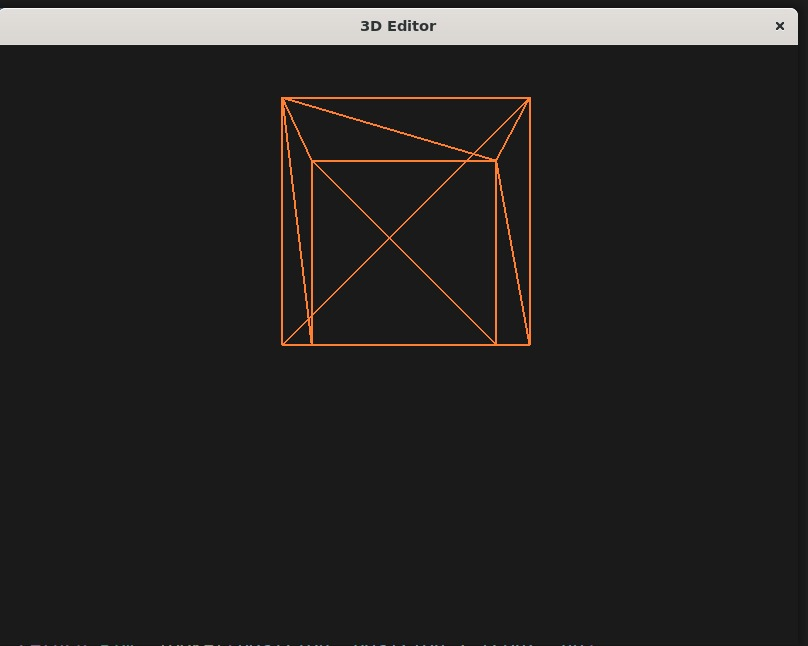
\includegraphics[width=0.5\textwidth]{ligne.jpeg}
    \caption{Cube triangular faces for rendering tests}
    \label{fig:cube_faces}
\end{figure} 

Regarding camera navigation, only WASD/ZQSD movement is currently implemented. Camera displacement is achieved by updating its position in 3D space based on user input. We also plan to add extra features such as zooming and camera rotation to improve the user experience.

\newpage

\section{Conclusion}

Most of the structural foundations of the project have been successfully established. However, several features still need to be developed to reach the final objectives. 

The primary difficulty encountered was our limited prior experience with C++, particularly regarding OpenGL and the various utility libraries. This required extra time to understand how they work and how to use them properly. 
Upcoming tasks include implementing mesh geometry editing, shortest path computation between arbitrary vertices, performance optimization, and robust error handling to prevent crashes.

\end{document}